% CHAPTER 3
\chapter{Materials and Methods}
\label{chp:chapter3}

\section{Datasets}

In this section we introduce the materials and datasets we use during our analysis. We took advantage of both experimental and computational approaches to identify RBP and miRNA sites in human 3'UTRs. Besides, we utilized datasets containing mRNA secondary structure information. At last, we used PTR datasets to assess the effect of trans-acting factors on stability and fate of transcripts.

\subsection{RNAcompete }

Determining the binding specificities of RBPs is the first critical phase to analysis their mechanism in PTR. We need large number of highly reliable binding sites to investigate their interaction with each other and to train models to be able to reason based on them.

RNAcompete is an \textit{in vitro} method for rapid and systematic analysis of RNA sequence preferences of RBPs \cite{rnacompete_09}. It characterized the binding specificities of more than 200 RPPs from 24 diverse eukaryotes. They tested the performance of RNAcompete by nine various RBPs and demonstrated that in most cases RNAcompete motifs are generally both accurate and functionally relevant. The method is able to identify previously known binding preferences along with novel ones. In this thesis we used RNAcompete to map RBP sites in human 3'UTRs.


\subsection{CLIP experiments and datasets}

In addition to \textit{in vitro} methods, we needed to take advantage of high resolution experimental methods to further confirm binding sites of RBPs. We downloaded CLIP-seq and PARCLIP data for a list of RBPs (HuR, FMR1, FUS, FXR1, FXR2, HNRNPA1, HNRNPA2B1, HNRNPC, IGF2BP1-3, LIN28, PUM2, QKI, SRSF1, TDP-43, TIA1, TIAL1) from doRINA database \cite{dorina_11}. In addition to these RBP specific CLIP datasets, we used gPARCLIP-determined peaks which provided information about genome-wide protein-occupied regions bound by any RBP in HEK293T cells. In contrast to global PARCLIP method, PARCLIP technique gives binding site specificities of particular RBP in specific transcript. We utilized both of these techniques to detect RBP binding sites with great accuracy. In a recent study by Friedersdorf and coworkers, they identified a background binding bias in CLIP-based techniques \cite{friedersdorf_14}. The technique discussed in that study, detects false-positive binding sites. These false-positive binding sites have been reducing efficiency of CLIP-based techniques. Removing those binding sites, significantly improve CLIP methods result. In order to abolish this bias, we excluded these regions from the CLIP peaks.

%explain about AGO proteins ant the role and then state from where (dorina) we downloaded AGO1-4 parclip, ago2 clip-seq and ago2-mnase parclip. 

\subsection{PhastCons conservation scores}

Protein binding sites are more likely to be conserved across species. Conservation score for a specific region of a transcript, represents the possibility of that region to be conserved in other species. There are two main algorithms which calculate conservation scores. The first one is PhastCons score which is the probability that each nucleotide belongs to a conserved element \cite{siepel_05}. Phylop is another existing method for detecting nucleotide substitution rates that are faster or slower than expected under neutral drift (cite Pylop). In our analysis we used PhastCons conservation scores (phastCons100way track downloaded from UCSC Genome Browser).

\subsection{TargetScan and PICTAR prediction methods}

There has been a lack of high-throughput biological and experimental approaches to detect the binding sites of miRNAs. In order to solve this issue, we took advantage of using computational methods such as TargetScan \cite{targetscan_05} and PicTar \cite{pictar_05} to identify putative miRNA target sites. TragetScan algorithm predicts miRNA target sites by searching 7-mer or 8-mer conserved regions that match the seed region of miRNAs (small 6-8 nucleotides long region at the 5' end of miRNAs). We also downloaded the predicted sites from PicTar algorithm. Structure and sequence are two important predictor of binding sites. These two computational methods focus on complementary with seed region and then analyze the thermodynamics for further improvements. In our analysis for each miRNAs site, we kept the data that whether it is supported by TargetScan and/or Pictar algorithms or not. Figure \ref{overview} illustrates the methods and datasets we used to map trans-acting factor binding sites.

\subsection{miRTARBase experimental method}

In addition to computational methods, we needed an other experimentally validated datasets in order to accredit our analysis results. Among several experimental methods, we decided to use miRTarBase \cite{mirtarbase} because it contained largest amount of miRNA-target interactions compared to other experimental datasets. Basically MirTarBase algorithm validates the miRNAs binding sites by reporter assays, western blot, or microarray experiments by overexpression or knockdown of miRNAs.

The interactions in miRTarBase database do not specify the exact position of miRNA target sites in mRNAs. However they only show that there are interaction between a particular miRNA and mRNA. Therefore, when there is a miRNA-mRNA interaction in the miRTarBase database, we assume that there is a target for that particular miRNA on that specific mRNA.


\subsection{SFOLD and RNAplfold}

Sequence and structure of RNAs are two important keys in understanding their function. The first step toward determining structure is to verify the RNA sequences. Recent developments in high-throughput sequencing techniques enabled researches to access invaluable genome-wide nucleotide sequences. However there is little knowledge about structure of RNAs. Many complex factors play role in determining the exact structure of RNAs. There are significant obstacles in front of verifying the secondary structures. First we should note that sequence length limits the RNA folding because of high memory consumption. On the other hand, the transcripts boundaries are not very well known. Because of these reasons, recent methods have tried to determine secondary structures in a given window size of \textit{L}. RNAplfold is one of the methods which uses local folding to calculate the base-pair probabilities \cite{RNAplfold}. For each base-pair, the probability is averaged over all windows of size \textit{L} that contained it. This algorithm uses little amount of memory and CPU time to run and therefore it is practical to scan large scale of genome for short RNA structure. The output of this method is a dot plot transcript file. Figure \ref{overview} represents a sample line of this file. The corresponding opening and closing parenthesis in each line represents a base-pair and dots stand for nucleotides without any complementary pair. 

% expand sfold as much as you can
There is another algorithm called SFOLD which generates a statistical sample of RNA secondary structures from the Boltzmann ensemble of RNA secondary structures \cite{sfold}. The Boltzmann distribution is measure of particles in a system over various possible states. SFOLD algorithm samples secondary structures strictly according to the Boltzmann distribution. It uses recent Turner free energy rules. We utilized this algorithm as a quantitative metric to further filter output of RNAplfold method.

\begin{figure*}[ht!]
   \centering
   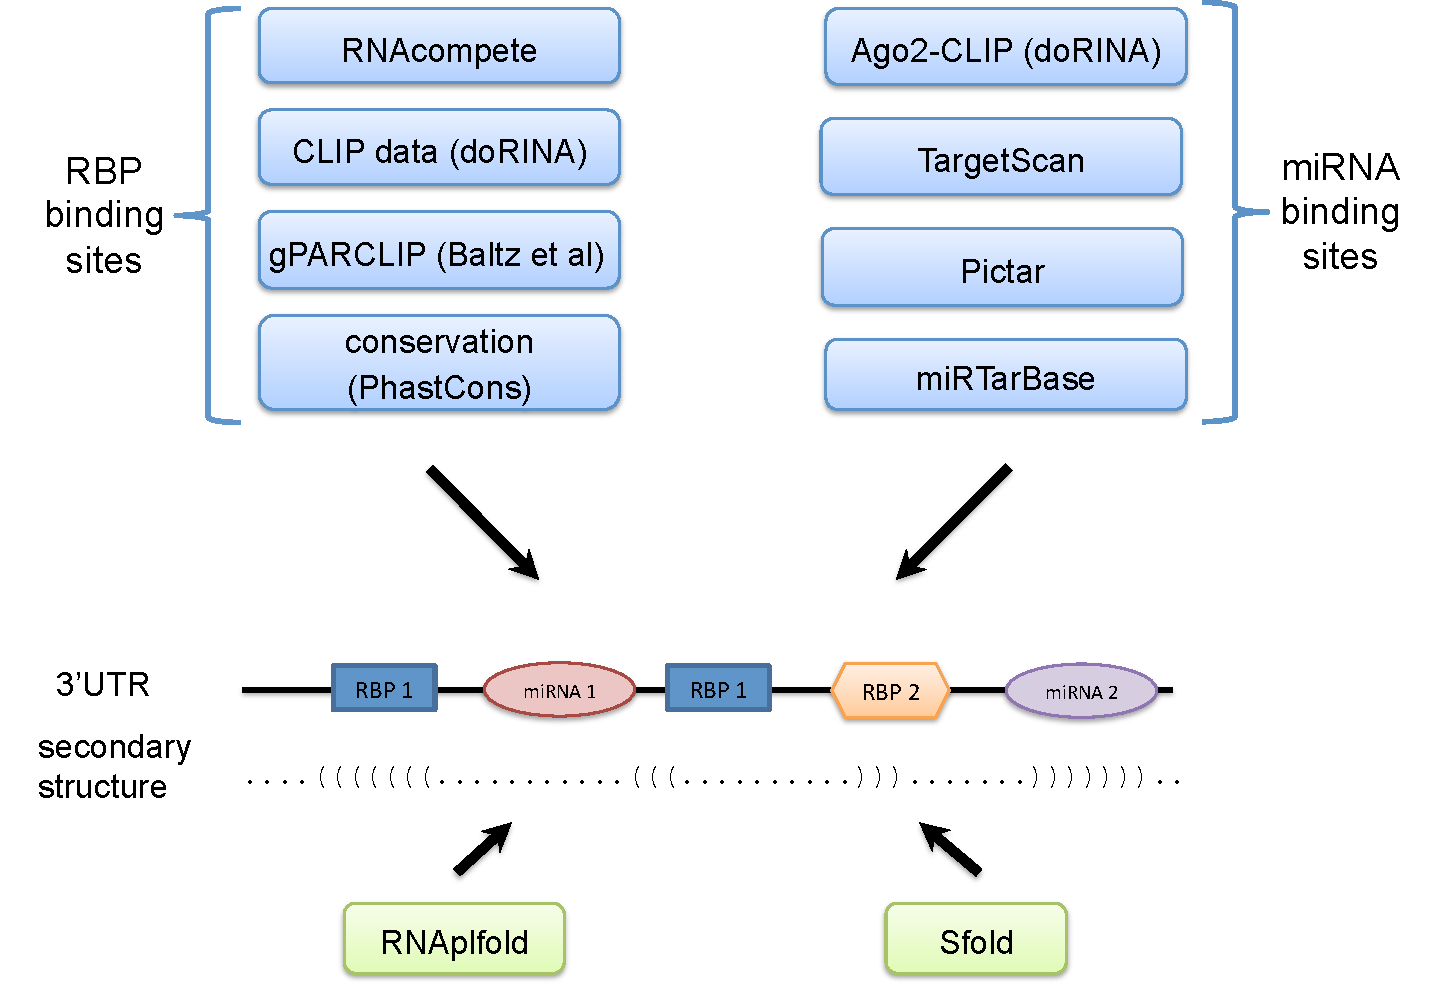
\includegraphics[width=0.8\textwidth,clip]{ch3_materials_methods/figures/Figure1.pdf}

\caption[]{Mapping of RBP and miRNA binding sites on human 3'UTRs. RBP binding sites are mapped by leveraging RNAcompete PFMs, CLIP- and PARCLIP-determined peaks and PhastCons conservation scores. miRNA binding sites are mapped by combining TargetScan and PicTar predictions with Ago-CLIP datasets and experimentally-verified interactions in miRTarBase database. Also, the secondary structure of the 3'UTRs are predicted with RNAplfold and Sfold. In particular, accessibility of a site is calculated by RNAplfold, and the probability of a site to form a stem-loop by binding to another site is calculated by Sfold.}
\label{overview}
\end{figure*}


\subsection{Datasets related to post-transcriptional regulation}

In order to analyze the effect of PTR trans-acting factors, we need to interpret related datasets. Knockdown and overexpression datasets are useful when we want to investigate the effect of particular factor in its depletion or abundance. In addition to these datasets, half-life and stability measurements represent mRNAs fate. In our analysis we used several post-transcriptional regulation datasets which are listed below:

\subsubsection{Knockdown datasets} We downloaded the Log fold changes (LFCs) of transcripts abundance upon HuR knockdown in HEK293 and HeLa cells from \cite{mukharjee_11} and \cite{lebedeva_11} respectively. These datasets helped us to investigate the effect of particular factor (HuR here) in PTR.

\subsubsection{Zhao dataset} In a recent study by Zhao and coworkers, they measured the effect of 3000 mRNA segments (160nts long) on mRNA stability and steady-state mRNA abundance in human BEAS-2B human bronchial epithelial cells \cite{zhao_14}. These mRNA segments were collected from 2089 human mRNA 3'UTRs. We downloaded the datasets from paper's supplementary data. The segments positions were given in hg18 genome which we converted into hg19 before using them. For each segment we specified from which mRNA it was selected.

\subsubsection{Schueler dataset} We downloaded mRNA half-lives measured in HEK293 and MCF7 cells \cite{schueler_14}. Unlike the knockdown and transfection datasets, half-live measurements help to investigate the effect of various factors in mRNA fate. It is beneficial to use these datasets to assay the effect of very well studied factors which we know they either promote or downregulate mRNA stability. With comparing situations in which a particular factor knocked down or over expressed, we will be able to see its effect easier.

It is known that the set of RBPs and miRNAs which are expressed in cell lines differ greatly between each cell type. Keeping this in mind, for each cell line discussed in our analysis, we determined the expressed factors in that particular cell line and used them in our further analysis. We used following sources to define the set of expressed RBPs and miRNAs in a given cell type:

\begin{itemize}
\item HEK293 cells: 
\begin{itemize}
\item RBPs: quantitative mass spectrometry results \cite{baltz_12}.
\item miRNAs: top 100 expressed miRNAs identified with small-RNA sequencing \cite{hafner_10}.
\end{itemize}
\item HeLa cells:
\begin{itemize}
\item RBPs: immunohistochemistry results from Human Protein Atlas database (http://www.proteinatlas.org).
\item miRNAs: top 100 expressed miRNAs identified with small-RNA sequencing \cite{lebedeva_11}.
\end{itemize}
\item MCF7 cells:
\begin{itemize}
\item RBPs: immunohistochemistry results from Human Protein Atlas database.
\item miRNAs: top 100 expressed miRNAs identified with small-RNA sequencing \cite{anbalagan_14}.
\end{itemize}
\item BEAS-2B cells:
\begin{itemize}
\item RBPs: immunohistochemistry results from Human Protein Atlas database.
\item miRNAs:  top 100 expressed miRNAs identified with small-RNA sequencing \cite{zhao_14}.
\end{itemize}
\end{itemize}

%write the reason why we prefered baltz over HPA.
We used Human Protein Atlas database for all mentioned cells except the HEK293 cells. The reason was that in Baltz paper, they performed quantitative mass spectrometry in HEK293 cells and their result is biologically validated (I am not sure about this reason, research). We also determined expressed RBPs in HEK293 cells using Human Protein Atlas. There was great correlation between expressed RBPs from Human Protein Atlas and quantitative mass spectrometry results (\%93.48 of expressed RBPs in Baltz et al. are same with Human Protein Atlas). 
%give more statistics about number of expressed factors in cells
For datasets that contain measurements mapped to gene IDs other than human RefSeq transcript IDs, we used the Synergizer tool for ID conversion \cite{synergizer}.

\section{Methods}

We used the datasets and algorithms from previous section to map the binding sites of RBPs and miRNAs in initial step and then utilized that collection to better understand PTR network. In the following sections, we introduce how we used computational and experimental methods to map trans-acting factor binding sites. Then we describe procedures in predicting RNA secondary structure of binding sites. At last, we introduce the statistical tests we used to assess our results' significance.

\subsection{Mapping RBP binding sites}

In order to map the binding sites of RBPs, we downloaded 103 position frequency matrices (PFMs) that correspond to 85 human RBPs from RNAcompete paper \cite{rnacompete_13}. These PFMs (which are of length seven or eight) are generated from the alignment of top 10 7-mers determined using all data (i.e. both setA and setB of RNAcompete pool). In order to represent motifs that are longer than seven nucleotide, we didn't use these top 10 7-mers directly and instead generated top 10 n-mers from these PFMs. In addition to RNAcompete motifs, we downloaded the motifs for the following well-known RBPs from RBPDB database \cite{rbpdb_11}: HNRNPAB, PUM1, PUM2, ELAVL2, KHSRP, ZFP36, AUF1 and CUGBP. Next, we determined binding sites of each RBP, by matching its top 10 n-mers or consensus motifs on human 3'UTR sequences. We downloaded human 3'UTR sequences from UCSC Genome Browser (on February 16th, 2014). 

%As a follow-up, we intersected the CLIP peaks with human 3'UTRs in order to determine experimentally validated binding sites. Finally, we excluded background binding regions from CLIP peaks to avoid the bias introduced by those false-positive targets.
After determining the binding sites of RBPs from previous step, we intersected them by CLIP peaks to detect experimentally validated sites. In this step, we also excluded the background bindings from CLIP peaks to avoid the bias caused by them.

Briefly, for each putative RBP binding site we keep the following information: (i) the start and end position; (ii) a flag showing whether the site is located in a CLIP- or gPARCLIP-determined peak; and (iii) conservation score calculated as the average PhastCons score. Figure \ref{overview} illustrates the datasets we used to map RBP binding sites.


\subsection{Mapping miRNA binding sites}

To determine the binding sites of miRNAs we took advantage of TargeScan and PicTar methods. We used AGO1-4 PARCLIP, AGO2 CLIP-seq and AGO2-MNase PARCLIP datasets to further validate computational method results. We also excluded background bindings as we did for RBPs. We used miRTarBase method to experimentally validate miRNA-mRNA interactions.

For each putative miRNA binding site, we keep track of its start and end position, a flag showing whether the site is supported by TargetScan, PicTar or both, a flag showing whether it is supported by miRTarBase and a flag whether the site is located in CLIP- or PARCLIP-determined peaks. Figure \ref{overview} shows the datasets we used in this approach.

\subsection{Predicting the RNA secondary structure of binding sites}

%Last paraghraphs of this section is same with paper, I should edit them.
Predicting the RNA secondary structure of binding sites is one of the most important steps toward getting invaluable knowledge about their behaviors. It helps us to explain possible interactions between post-transcriptional regulatory factors. We predicted RNA secondary structure of human 3'UTRs with RNAplfold. We used output base-pair probabilities from this algorithm to determine accessibility. Namely, we calculated the average probability of being in unpaired context across the site. Next we classified the site as accessible if this value was greater than $0.6$ and inaccessible if the value was less than $0.4$. Being an accessible site means that it is possible for RBPs and miRNAs to bind to that site. On the other hand, an inaccessible site is not available for factors to bind to it. 

In a study by Lange and coworkers, they have shown that local folding with a window length of 200 and base pair span of 150 gives optimal results compared to using other parameters or even global folding \cite{lange_12}. Their findings suggests that local folding is more accurate than the classic global approach. Keeping this in mind, we applied local folding by running RNAplfold with the parameters -W 200 and -L 150 where '-W' specifies the length of the local window and '-L' restricts the maximal base pair span.

As in the interplay between PUM1-miR-221 (or miR-222), factors may cooperate with each other to regulate the transcript and express a vital effect on their stability. In the mentioned example, both PUM protein and miR-221(222) bind to two side of a same stem-loop and help each other to alter secondary structure of p27 genes' 3'UTR. Our main goal in this thesis is to discover similar interaction.

In order to identify similar potential cooperative interaction, first we need to know which binding sites may have interaction with each other. Our hypothesis is that the more base pairs that can be formed between two sites, the higher possibility there is that they may be in some kind of interaction between each other. At first step, we calculated the number of base pairs that can be formed between each pair of sites by considering only reverse complementarity. We assumed the pairs of sites with more than 5 base pairs as potential interactors.

One of the important issues which needs to be considered during this analysis is that a site can be reverse complementary to several other sites. In this case, we need to select the partner site which is most likely to form a stem-loop. For this reason, we need a quantitative metric to sort and weight the various possible complementary sites. We used SFOLD algorithm to generate 1000 sample structures from the Boltzmann distribution of all possible structures for each running window of length 200nt. For each pair of binding sites, we considered those windows that both sites are located in. Next, we parsed all the sampled structures of each window to calculate the average number of base pairs formed between the two sites. This value reflects the probability that the two sites will form a stem-loop.

As a follow up, we sorted the potential interacting site determined by reverse complementary according to possibilities calculated by SFOLD. In this step, we filtered out sites with probability less than 0.1 to clean our data. Then from top of the list which contained higher SFOLD possibilities, we selected unique pairs of sites and ignored alternative possible interacting sites of an already selected site. For example, let's assume that a particular 3'UTR contains three sites labeled as A, B and C, and each pair of these sites can form a stem-loop with more than $\geq 5$ base pairs. Let's also assume that the Sfold-calculated probabilities for these pairs are as follows: A-B: 0.3, B-C: 0.6, A-C: 0.4. With our procedure, B-C pair would score the highest and get selected, whereas A-B and A-C pairs would be ignored as B and C are already considered. Afterward, we considered the resulted dataset as our source to decide interacting sites in our analysis.

% change the following pharaghraphs too. 

\subsection{Testing for significance}

We used two-tailed Mann-Whitney U test (also called Wilcoxon rank-sum test) to compare various properties (e.g.
log fold change, stability) of sets of transcripts (see Results section), and we used Wilcoxon signed-rank test to compare the area under the ROC curve (AUROC) values of different logistic regression models.


\subsection{Predicting stability and expression using logistic regression}

To run logistic regression with L2 regularization, we used the glmnet package \cite{glmnet} with alpha parameter set to 0. Within each cross-validation run, we ran the \textit{cv.glmnet} function to determine the optimal lambda (i.e. regularization constant) value.
